% Options for packages loaded elsewhere
\PassOptionsToPackage{unicode}{hyperref}
\PassOptionsToPackage{hyphens}{url}
\PassOptionsToPackage{dvipsnames,svgnames,x11names}{xcolor}
\documentclass[
  10pt,
  fontset=fandol]{ctexart}
\usepackage{xcolor}
\usepackage[margin=16mm]{geometry}
\usepackage{amsmath,amssymb}
\setcounter{secnumdepth}{-\maxdimen} % remove section numbering
\usepackage{iftex}
\ifPDFTeX
  \usepackage[T1]{fontenc}
  \usepackage[utf8]{inputenc}
  \usepackage{textcomp} % provide euro and other symbols
\else % if luatex or xetex
  \usepackage{unicode-math} % this also loads fontspec
  \defaultfontfeatures{Scale=MatchLowercase}
  \defaultfontfeatures[\rmfamily]{Ligatures=TeX,Scale=1}
\fi
\usepackage{lmodern}
\ifPDFTeX\else
  % xetex/luatex font selection
\fi
% Use upquote if available, for straight quotes in verbatim environments
\IfFileExists{upquote.sty}{\usepackage{upquote}}{}
\IfFileExists{microtype.sty}{% use microtype if available
  \usepackage[]{microtype}
  \UseMicrotypeSet[protrusion]{basicmath} % disable protrusion for tt fonts
}{}
\makeatletter
\@ifundefined{KOMAClassName}{% if non-KOMA class
  \IfFileExists{parskip.sty}{%
    \usepackage{parskip}
  }{% else
    \setlength{\parindent}{0pt}
    \setlength{\parskip}{6pt plus 2pt minus 1pt}}
}{% if KOMA class
  \KOMAoptions{parskip=half}}
\makeatother
\usepackage{longtable,booktabs,array}
\newcounter{none} % for unnumbered tables
\usepackage{calc} % for calculating minipage widths
% Correct order of tables after \paragraph or \subparagraph
\usepackage{etoolbox}
\makeatletter
\patchcmd\longtable{\par}{\if@noskipsec\mbox{}\fi\par}{}{}
\makeatother
% Allow footnotes in longtable head/foot
\IfFileExists{footnotehyper.sty}{\usepackage{footnotehyper}}{\usepackage{footnote}}
\makesavenoteenv{longtable}
\usepackage{graphicx}
\makeatletter
\newsavebox\pandoc@box
\newcommand*\pandocbounded[1]{% scales image to fit in text height/width
  \sbox\pandoc@box{#1}%
  \Gscale@div\@tempa{\textheight}{\dimexpr\ht\pandoc@box+\dp\pandoc@box\relax}%
  \Gscale@div\@tempb{\linewidth}{\wd\pandoc@box}%
  \ifdim\@tempb\p@<\@tempa\p@\let\@tempa\@tempb\fi% select the smaller of both
  \ifdim\@tempa\p@<\p@\scalebox{\@tempa}{\usebox\pandoc@box}%
  \else\usebox{\pandoc@box}%
  \fi%
}
% Set default figure placement to htbp
\def\fps@figure{htbp}
\makeatother
\setlength{\emergencystretch}{3em} % prevent overfull lines
\providecommand{\tightlist}{%
  \setlength{\itemsep}{0pt}\setlength{\parskip}{0pt}}
\usepackage{amsmath,amssymb,mathtools,needspace}
\xeCJKDeclareCharClass{CJK}{"2032,"0400->"04FF,"2160->"216B,"2460->"2473,"25A0,"25C7,"25CB,"25CF}
\IfFontExistsTF{Arial Unicode MS}{\xeCJKsetup{AutoFallBack=true}\setCJKfallbackfamilyfont{\CJKrmdefault}{Arial Unicode MS}}{}
\setcounter{secnumdepth}{0}
\setlength{\emergencystretch}{2em}
\allowdisplaybreaks
\usepackage{bookmark}
\IfFileExists{xurl.sty}{\usepackage{xurl}}{} % add URL line breaks if available
\urlstyle{same}
\hypersetup{
  pdftitle={逐次线性插值法},
  colorlinks=true,
  linkcolor={Maroon},
  filecolor={Maroon},
  citecolor={Blue},
  urlcolor={Blue},
  pdfcreator={LaTeX via pandoc}}

\title{逐次线性插值法}
\author{}
\date{}

\begin{document}
\maketitle

\subsection{2.3 逐次线性插值法}\label{ux9010ux6b21ux7ebfux6027ux63d2ux503cux6cd5}

用 Lagrange 插值多项式 \(L_n(x)\) 计算函数近似值时，如需增加插值节点，那么原来算出的数据均不能利用，必须重新计算。为克服这个缺点，通常可用逐次线性插值方法求得高次插值。如例 2.1 中 \(L_2(0.336\,7)\) 是由式（2.2.7）计算的，它也可由 \(L_1(0.336\,7)\) 和 \(\widetilde L_1(0.336\,7)\) 按类似线性插值的方法计算，即

\[
\begin{aligned}
L_2(0.336\,7)
&=L_1(0.336\,7)
+\frac{\widetilde L_1(0.336\,7)-L_1(0.336\,7)}{0.36-0.32}
\times(0.336\,7-0.32)\\
&=0.330\,365+\frac{0.000\,022}{0.04}\times0.016\,7\\
&=0.330\,374.
\end{aligned}
\]

\subsubsection{校注（agent 补充）：NA5E-E002}\label{ux6821ux6ce8agent-ux8865ux5145na5e-e002}

上面的 \(0.828\)、\(0.178\times10^{-7}\) 和代入行的 \(3.89\times10^{-4}\) 均经过原页放大核对，确为扫描原书印字。\textbf{这几行不能直接作为正确的数值结果使用。}

\begin{enumerate}
\def\labelenumi{\arabic{enumi}.}
\tightlist
\item
  本例以弧度计算，\(\cos0.32\approx0.9492354180824409\)，所以 \(\cos x_0<0.828\) 不成立。可用保守上界 \(M_3<0.95\)。
\item
  即使照原书使用 \(0.828\)，该乘积也等于 \(1.77200694\times10^{-7}\)，大于原文所写的 \(0.178\times10^{-7}=1.78\times10^{-8}\)。
\item
  对正确的导数上界，用原节点得到的截断误差上界为
\end{enumerate}

\[
|R_2(0.3367)|
\le\frac{0.95}{6}\,(0.0167)(0.0033)(0.0233)
=2.03309975\times10^{-7}.
\]

这里的 \(R_2\) 指用精确节点函数值定义的插值截断误差。

\begin{enumerate}
\def\labelenumi{\arabic{enumi}.}
\setcounter{enumi}{3}
\tightlist
\item
  二次插值代入行的中间乘积应为 \(0.0167\times0.0233=0.00038911=3.8911\times10^{-4}\)。若严格按原书印出的 \(3.89\times10^{-4}\) 计算整行，会得到 \(0.3302826531125\)，不能得到末行的 \(0.330374\)。保留精确乘积，并使用题目给的有限精度表值，可得
\end{enumerate}

\[
\begin{aligned}
L_1(0.3367)&=0.3303652,\\
\widetilde L_1(0.3367)&=0.330387145,\\
L_2(0.3367)&=0.3303743620375.
\end{aligned}
\]

最后一项保留六位有效数字确实为 \(0.330374\)，与 \(\sin0.3367\approx0.3303741915556280\) 的六位有效数字一致。

\href{../../source-images/pdf-035.jpeg}{原页：书页 22／PDF 35}

\begin{quote}
本页末句续 PDF 36。
\end{quote}

现令 \(I_{i_1,i_2,\cdots,i_n}(x)\) 表示函数 \(f(x)\) 关于节点 \(x_{i_1},x_{i_2},\cdots,x_{i_n}\) 的 \(n-1\) 次插值多项式，\(I_{i_k}(x)\) 是零次多项式，记 \(I_{i_k}(x)=f(x_{i_k})\)，\(i_1,i_2,\cdots,i_n\) 均为非负整数。一般情况，两个 \(k\) 次插值多项式可通过线性插值得到 \(k+1\) 次插值多项式

\[
I_{0,1,\cdots,k,l}(x)
=I_{0,1,\cdots,k}(x)
+\frac{I_{0,1,\cdots,k-1,l}(x)-I_{0,1,\cdots,k}(x)}
{x_l-x_k}(x-x_k).
\tag{2.3.1}
\]

这是关于节点 \(x_0,\cdots,x_k,x_l\) 的插值多项式。显然

\[
I_{0,1,\cdots,k,l}(x_i)=I_{0,1,\cdots,k}(x_i)=f(x_i)
\]

对于 \(i=0,1,\cdots,k-1\) 成立。当 \(x=x_k\) 时，有

\[
I_{0,1,\cdots,k,l}(x_k)=I_{0,1,\cdots,k}(x_k)=f(x_k),
\]

当 \(x=x_l\) 时，有

\[
\begin{aligned}
I_{0,1,\cdots,k,l}(x_l)
&=I_{0,1,\cdots,k}(x_l)
+\frac{f(x_l)-I_{0,1,\cdots,k}(x_l)}{x_l-x_k}(x_l-x_k)\\
&=f(x_l).
\end{aligned}
\]

这就证明了式（2.3.1）的插值多项式满足插值条件，称式（2.3.1）为 \textbf{Aitken 逐次线性插值公式}。当 \(k=0\) 时为线性插值。当 \(k=1\) 时插值节点为 \(x_0,x_1,x_l\)，插值多项式为

\[
I_{0,1,l}(x)=I_{0,1}(x)
+\frac{I_{0,l}(x)-I_{0,1}(x)}{x_l-x_1}(x-x_1).
\]

计算时可由 \(k=0\) 到 \(k=n-1\) 逐次求得所需的插值多项式，计算过程如表 2.1 所示。

\textbf{表 2.1}

\begin{quote}
表中``节点／函数值／1 次至 4 次／原表最右列''为 agent 添加的列名；原表无表头，以下保留全部单元格。
\end{quote}

{\def\LTcaptype{none} % do not increment counter
\begin{longtable}[]{@{}
  >{\raggedright\arraybackslash}p{(\linewidth - 12\tabcolsep) * \real{0.1429}}
  >{\raggedright\arraybackslash}p{(\linewidth - 12\tabcolsep) * \real{0.1429}}
  >{\raggedright\arraybackslash}p{(\linewidth - 12\tabcolsep) * \real{0.1429}}
  >{\raggedright\arraybackslash}p{(\linewidth - 12\tabcolsep) * \real{0.1429}}
  >{\raggedright\arraybackslash}p{(\linewidth - 12\tabcolsep) * \real{0.1429}}
  >{\raggedright\arraybackslash}p{(\linewidth - 12\tabcolsep) * \real{0.1429}}
  >{\raggedright\arraybackslash}p{(\linewidth - 12\tabcolsep) * \real{0.1429}}@{}}
\toprule\noalign{}
\begin{minipage}[b]{\linewidth}\raggedright
节点
\end{minipage} & \begin{minipage}[b]{\linewidth}\raggedright
函数值
\end{minipage} & \begin{minipage}[b]{\linewidth}\raggedright
1 次
\end{minipage} & \begin{minipage}[b]{\linewidth}\raggedright
2 次
\end{minipage} & \begin{minipage}[b]{\linewidth}\raggedright
3 次
\end{minipage} & \begin{minipage}[b]{\linewidth}\raggedright
4 次
\end{minipage} & \begin{minipage}[b]{\linewidth}\raggedright
原表最右列
\end{minipage} \\
\midrule\noalign{}
\endhead
\bottomrule\noalign{}
\endlastfoot
\(x_0\) & \(f(x_0)=I_0\) & & & & & \(x-x_0\) \\
\(x_1\) & \(f(x_1)=I_1\) & \(I_{0,1}\) & & & & \(x-x_1\) \\
\(x_2\) & \(f(x_2)=I_2\) & \(I_{0,2}\) & \(I_{0,1,2}\) & & & \(x-x_2\) \\
\(x_3\) & \(f(x_3)=I_3\) & \(I_{0,3}\) & \(I_{0,1,3}\) & \(I_{0,1,2,3}\) & & \(x-x_3\) \\
\(x_4\) & \(f(x_4)=I_4\) & \(I_{0,4}\) & \(I_{0,1,4}\) & \(I_{0,1,2,4}\) & \(I_{0,1,2,3,4}\) & \(x-x_4\) \\
\end{longtable}
}

式（2.3.1）也可改为以下计算公式：

\[
I_{0,1,\cdots,k+1}(x)
=I_{0,1,\cdots,k}(x)
+\frac{I_{1,2,\cdots,k+1}(x)-I_{0,1,\cdots,k}(x)}
{x_{k+1}-x_0}(x-x_0),
\tag{2.3.2}
\]

并称它为 \textbf{Neville 算法}，其计算过程如表 2.2 所示。

\textbf{表 2.2}

\begin{quote}
表中列名为 agent 添加；原表以斜线联结 \(I_{0,1}\)、\(I_{0,1,2}\)、\(I_{0,1,2,3}\)、\(I_{0,1,2,3,4}\)。最右列首行原印为 \(x-x_0\)，其后为 \(x_i-x_0\)。
\end{quote}

{\def\LTcaptype{none} % do not increment counter
\begin{longtable}[]{@{}
  >{\raggedright\arraybackslash}p{(\linewidth - 12\tabcolsep) * \real{0.1429}}
  >{\raggedright\arraybackslash}p{(\linewidth - 12\tabcolsep) * \real{0.1429}}
  >{\raggedright\arraybackslash}p{(\linewidth - 12\tabcolsep) * \real{0.1429}}
  >{\raggedright\arraybackslash}p{(\linewidth - 12\tabcolsep) * \real{0.1429}}
  >{\raggedright\arraybackslash}p{(\linewidth - 12\tabcolsep) * \real{0.1429}}
  >{\raggedright\arraybackslash}p{(\linewidth - 12\tabcolsep) * \real{0.1429}}
  >{\raggedright\arraybackslash}p{(\linewidth - 12\tabcolsep) * \real{0.1429}}@{}}
\toprule\noalign{}
\begin{minipage}[b]{\linewidth}\raggedright
节点
\end{minipage} & \begin{minipage}[b]{\linewidth}\raggedright
函数值
\end{minipage} & \begin{minipage}[b]{\linewidth}\raggedright
1 次
\end{minipage} & \begin{minipage}[b]{\linewidth}\raggedright
2 次
\end{minipage} & \begin{minipage}[b]{\linewidth}\raggedright
3 次
\end{minipage} & \begin{minipage}[b]{\linewidth}\raggedright
4 次
\end{minipage} & \begin{minipage}[b]{\linewidth}\raggedright
原表最右列
\end{minipage} \\
\midrule\noalign{}
\endhead
\bottomrule\noalign{}
\endlastfoot
\(x_0\) & \(f(x_0)=I_0\) & & & & & \(x-x_0\) \\
\(x_1\) & \(f(x_1)=I_1\) & \(I_{0,1}\) & & & & \(x_1-x_0\) \\
\(x_2\) & \(f(x_2)=I_2\) & \(I_{1,2}\) & \(I_{0,1,2}\) & & & \(x_2-x_0\) \\
\(x_3\) & \(f(x_3)=I_3\) & \(I_{2,3}\) & \(I_{1,2,3}\) & \(I_{0,1,2,3}\) & & \(x_3-x_0\) \\
\(x_4\) & \(f(x_4)=I_4\) & \(I_{3,4}\) & \(I_{2,3,4}\) & \(I_{1,2,3,4}\) & \(I_{0,1,2,3,4}\) & \(x_4-x_0\) \\
\end{longtable}
}

从表 2.2 看到：每增加一个节点就计算一行，斜线上是 1 次到 4 次插值多项式的

\begin{quote}
转录核对说明（agent 补充）：表 2.2 首行最右格已据原图放大核为 \(x-x_0\)，纠正既有章节转录的 \(x_0-x_0\)；这属于转录错误，不是原书校勘。
\end{quote}

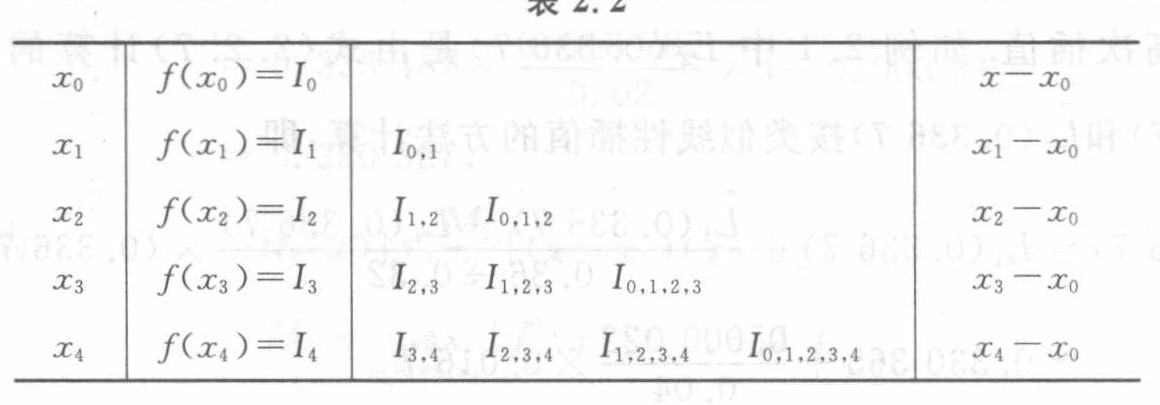
\includegraphics[width=0.85\linewidth,height=\textheight,keepaspectratio,alt={表 2.2 原图核对裁切}]{../assets/ch02a/pdf-035-table-2.2-detail.png}

\href{../../source-images/pdf-036.jpeg}{原页：书页 23／PDF 36}

\begin{quote}
页首接 PDF 35 的``插值多项式的''。
\end{quote}

值；如精度不满足要求，再增加一个节点，前面计算完全有效。这个算法适用于在计算机上计算，且具有自动选取节点并逐步比较精度的特点，程序也较简单。

\textbf{例 2.2} 已知 \(f(x)=\operatorname{sh}x\) 的值在表 2.3 左端，用 Aitken 插值求 \(\operatorname{sh}0.23\) 的近似值。

\textbf{解} 表 2.3 右端是各次插值的计算结果，由于 3 次插值的两个结果相同，因而不需再计算 4 次插值，故求得 \(f(0.23)=0.232\,034\)。

\textbf{表 2.3}

\begin{quote}
原表表头为 \(x_i\)、\(f(x_i)\)、插值结果。左右数据在扫描中采用错行排布，以下分开排成可检索表；``1 次、2 次、3 次''为 agent 添加的列名。
\end{quote}

左端节点数据：

{\def\LTcaptype{none} % do not increment counter
\begin{longtable}[]{@{}rr@{}}
\toprule\noalign{}
\(x_i\) & \(f(x_i)\) \\
\midrule\noalign{}
\endhead
\bottomrule\noalign{}
\endlastfoot
\(0.00\) & \(0.000\,0\) \\
\(0.20\) & \(0.201\,34\) \\
\(0.30\) & \(0.304\,52\) \\
\(0.50\) & \(0.521\,10\) \\
\(0.60\) & \(0.636\,65\) \\
\end{longtable}
}

右端插值结果：

{\def\LTcaptype{none} % do not increment counter
\begin{longtable}[]{@{}rrr@{}}
\toprule\noalign{}
1 次 & 2 次 & 3 次 \\
\midrule\noalign{}
\endhead
\bottomrule\noalign{}
\endlastfoot
\(0.231\,54\) & & \\
\(0.233\,465\) & \(0.232\,118\) & \\
\(0.239\,706\) & \(0.232\,358\) & \(\underline{0.232\,034}\) \\
\(0.244\,049\) & \(0.232\,479\) & \(0.232\,034\) \\
\end{longtable}
}

\begin{center}\rule{0.5\linewidth}{0.5pt}\end{center}

\subsection{相关原页校注（agent 补充）}\label{ux76f8ux5173ux539fux9875ux6821ux6ce8agent-ux8865ux5145}

以下校注来自本节覆盖的原页，可能也涉及同页相邻小节；原文照录与校正说明分开保留。

\subsubsection{原书 PDF 页 36 的校注}\label{ux539fux4e66-pdf-ux9875-36-ux7684ux6821ux6ce8}

\href{../pages/pdf-036.md}{完整原页转录} · \href{../../source-images/pdf-036.jpeg}{原页图像}

\subsubsection{校注（agent 补充）：代入行的原书记号}\label{ux6821ux6ce8agent-ux8865ux5145ux4ee3ux5165ux884cux7684ux539fux4e66ux8bb0ux53f7}

上面``当 \(x=x_1\) 时''一行，扫描原书实际写成 \(a_0+a_1(x-x_0)\)，其中 \(x\) 没有下标 \(1\)，本转录予以保留。在该行已经限定的 \(x=x_1\) 条件下，求系数时即代入 \(x_1\)；不将这一记号静默改写成原文没有印出的 \(a_1(x_1-x_0)\)。原页的 \(a_2\) 分式有整体分母 \(x_2-x_1\)，OCR 漏掉了这一层分母，本转录已恢复。

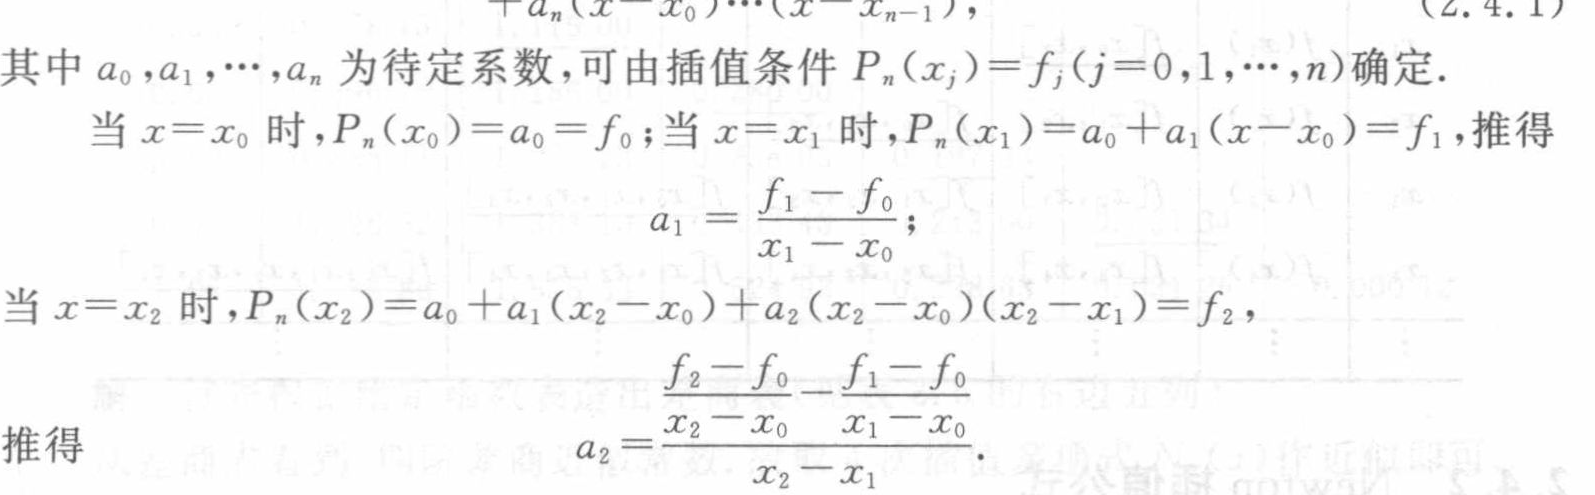
\includegraphics[width=0.85\linewidth,height=\textheight,keepaspectratio,alt={PDF 36 代入与系数原图裁切}]{../assets/ch02a/pdf-036-coefficients-detail.png}

\subsection{本节覆盖原页的校注记录}\label{ux672cux8282ux8986ux76d6ux539fux9875ux7684ux6821ux6ce8ux8bb0ux5f55}

下列记录按原页关联，含同页相邻小节的校注；计算时同时读取上文校注和完整原页。

\begin{itemize}
\tightlist
\item
  \texttt{NA5E-E002}：原书 PDF 页 34
\end{itemize}

\end{document}
